\section{Spécifications fonctionnelles}
	
\subsection{Conseils de prévention}
	L'application devra permettre de fournir à l'utilisateur des informations appropriées en fonction de sa situation.Par exemple, elles peuvent concerner les transports en commun, les lieux publics, les hôtels ou encore les urgences. Ces informations auront pour objectif de conseiller un touriste étranger en France sur la conduite à adopter et la manière d'appréhender les choses lorsque celui-ci se trouve dans une situation particulière. Ces conseils sont fournis sous forme de fiche au format odt par la gendarmerie. De plus, celle-ci souhaite pouvoir ajouter de nouvelles informations lorsqu'elle le désire. Cependant, les connaissances informatique du client étant limitées, l'application devra permettre un ajout simplifié de ces informations. Par exemple par simple dépôt d'une fiche au bon format dans un dossier. Les situations seront symbolisées sous forme de liste de pictogrammes explicites auxquels seront adjoints des mots clés.
	
\subsection{Contacts}

	L'application devra donner la possibilité à l'utilisateur d'accéder à une liste de contacts à appeler en cas d'urgence. Cette liste contiendra des numéros tels que ceux de la gendarmerie/police, des urgences, des pompiers ... Cette liste permettra de rediriger l'utilisateur sur son composeur téléphonique avec le numéro correspondant au contact qu'il souhaite appeler. Ainsi, celui-ci aura toujours le choix de confirmer ou d'annuler l'appel.
	
\subsection{Géolocalisation}

	L'application devra contenir un module de géolocalisation et de navigation permettant de guider l'utilisateur vers la destination de son choix. Elle proposera une liste de destinations pouvant être utiles en fonction de la situation du touriste comme la gendarmerie, le consulat ou l'hôpital. Cette fonctionnalité aura pour objectif de renvoyer l'utilisateur sur Google Maps avec une recherche pré-effectuée pointant sur la direction qu'il aura choisi.

\subsection{Profil}

	L'application devra permettre à l'utilisateur de pouvoir écrire ses informations personnelles ainsi que que les remarques médicales le concernant. Ces informations pourront être utilisées en cas d'urgence ou pour lister les différents problèmes concernant l'utilisateur

\subsection{Multilingue}

	L'application étant proposée à des touristes ou résidents étranger en France, celle-ci devra être multilingue. Les différents menus, listes de contacts et destinations seront donc traduits dans différentes langues. Les fiches de conseils devront également être traduites dans différentes langues. Elle devra proposer à l'utilisateur de choisir sa nationalité lors de sa première utilisation de l'application. De plus, elle devra également lui permettre de pouvoir modifier son choix et donc de changer de langue à tout moment.

\section{Cas d'utilisation}

	Le diagramme présent sur la figure \ref{casUtilisations} permet de représenter les différents cas d'utilisation de l'application.
	
\begin{figure}[!h]
	\begin{center}
	
		\includegraphics[scale=0.6]{images/casUtilisations.png}
	    \caption{Diagramme de Cas d'Utilisation}
	    \label{casUtilisations} 
	
	\end{center}
\end{figure}

\newpage

\section{Spécifications d'interfaces}
	Les images \ref{maquette1} et \ref{maquette2} représentent la maquette permettant de décrire le cahier des charges et les spécifications d'interface qui nous ont été fourni pour la réalisation de notre application.

\begin{figure}[H]
	\begin{center}
		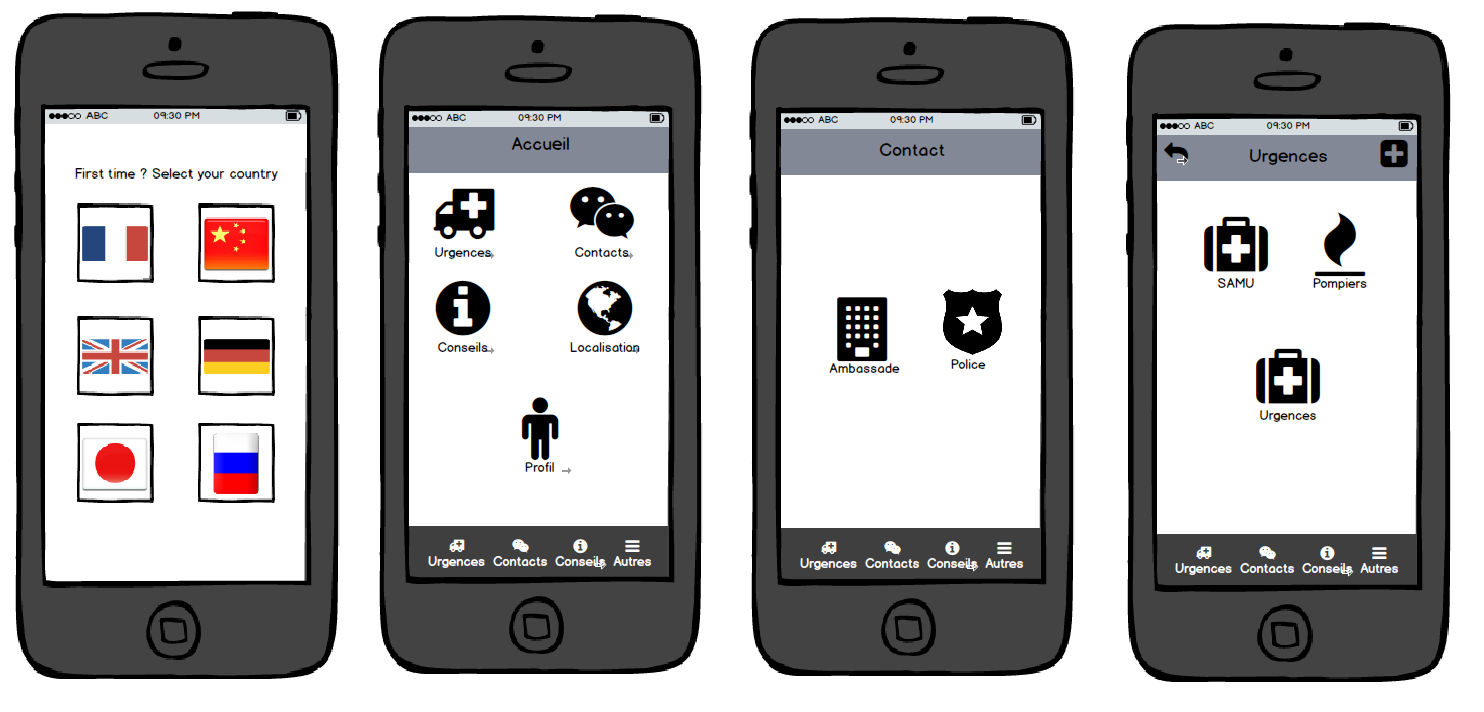
\includegraphics[scale=0.5]{images/maquette1.png}
		\caption{Maquette de l'application}
		\label{maquette1} 
		
	\end{center}
\end{figure}

\begin{figure}[H]
	\begin{center}
		
		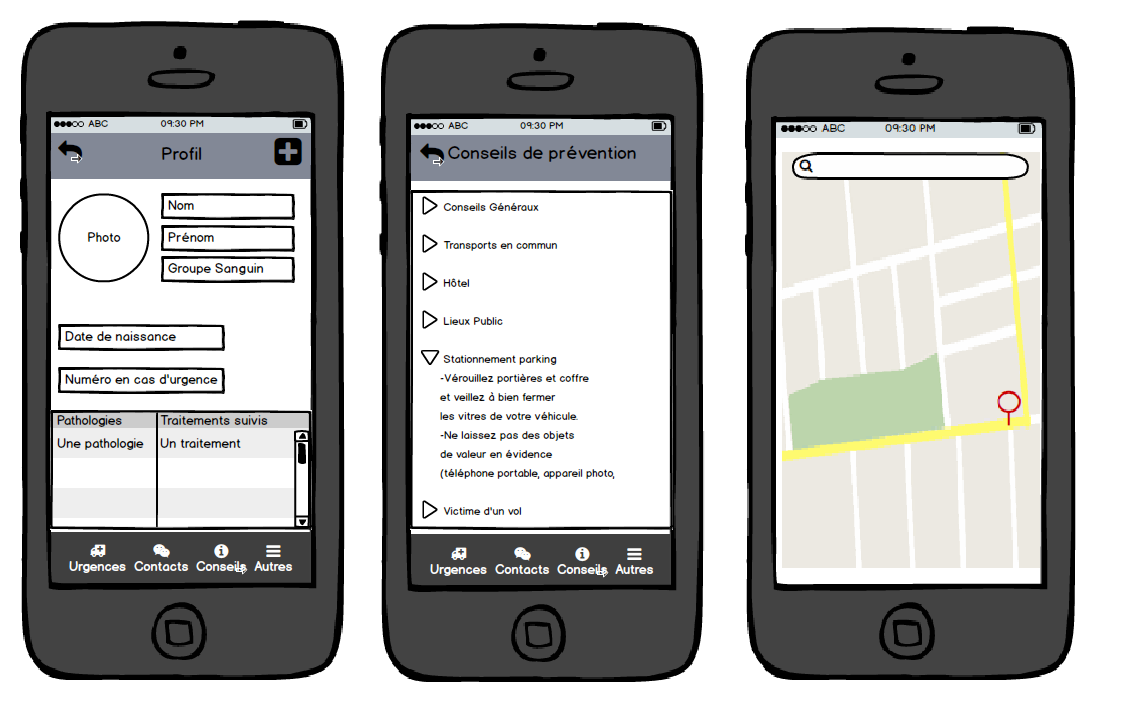
\includegraphics[scale=0.5]{images/maquette2.png}
		\caption{Maquette de l'application : }
		\label{maquette2} 
		
	\end{center}
\end{figure}

\section{Spécifications opérationnelles}

\subsubsection{Caractéristiques techniques}
	L'application sera fonctionnelle sous le système d'exploitation mobile Android en version 4.0 minimum. Celle-ci devra être fluide et adaptée à une utilisation tactile. Elle sera proposée à des  utilisateurs ayant des nationalités différentes c'est pourquoi elle devra être lisible et graphique.
	Cette application sera off-line c'est-à-dire sans échange de données direct. Dans le but d'utiliser le module de géolocalisation elle devra faire appel à une application tierce, Google Maps. En outre, elle sera responsive et donc en mesure de s'adapter à différents écrans.

\subsubsection{Permissions}

	L'application nécessitera plusieurs permissions dans l'optique que l'utilisateur puisse profiter pleinement de toutes ses fonctionnalités. Les permissions requises sont les suivantes : 
	\begin{itemize}
		\item \texttt{android.permission.CALL\_PHONE} Autorise l'application à rediriger l'utilisateur sur le composeur téléphonique en lui laissant le choix de confirmer ou non l'appel.
		\item \texttt{android.permission.READ\_EXTERNAL\_STORAGE} Autorise l'application à lire du contenu externe stocké sur le téléphone.
		\item \texttt{android.permission.ACCESS\_COARSE\_LOCATION} Autorise l'application à utiliser les fonctions de géolocalisation approximative.
		\item \texttt{android.permission.ACCESS\_FINE\_LOCATION} Autorise l'application à utiliser les fonctions de géolocalisation de haute précision.
	\end{itemize}	   	